\documentclass{standalone}
\usepackage{tikz}
\usetikzlibrary{patterns, positioning}


\begin{document}
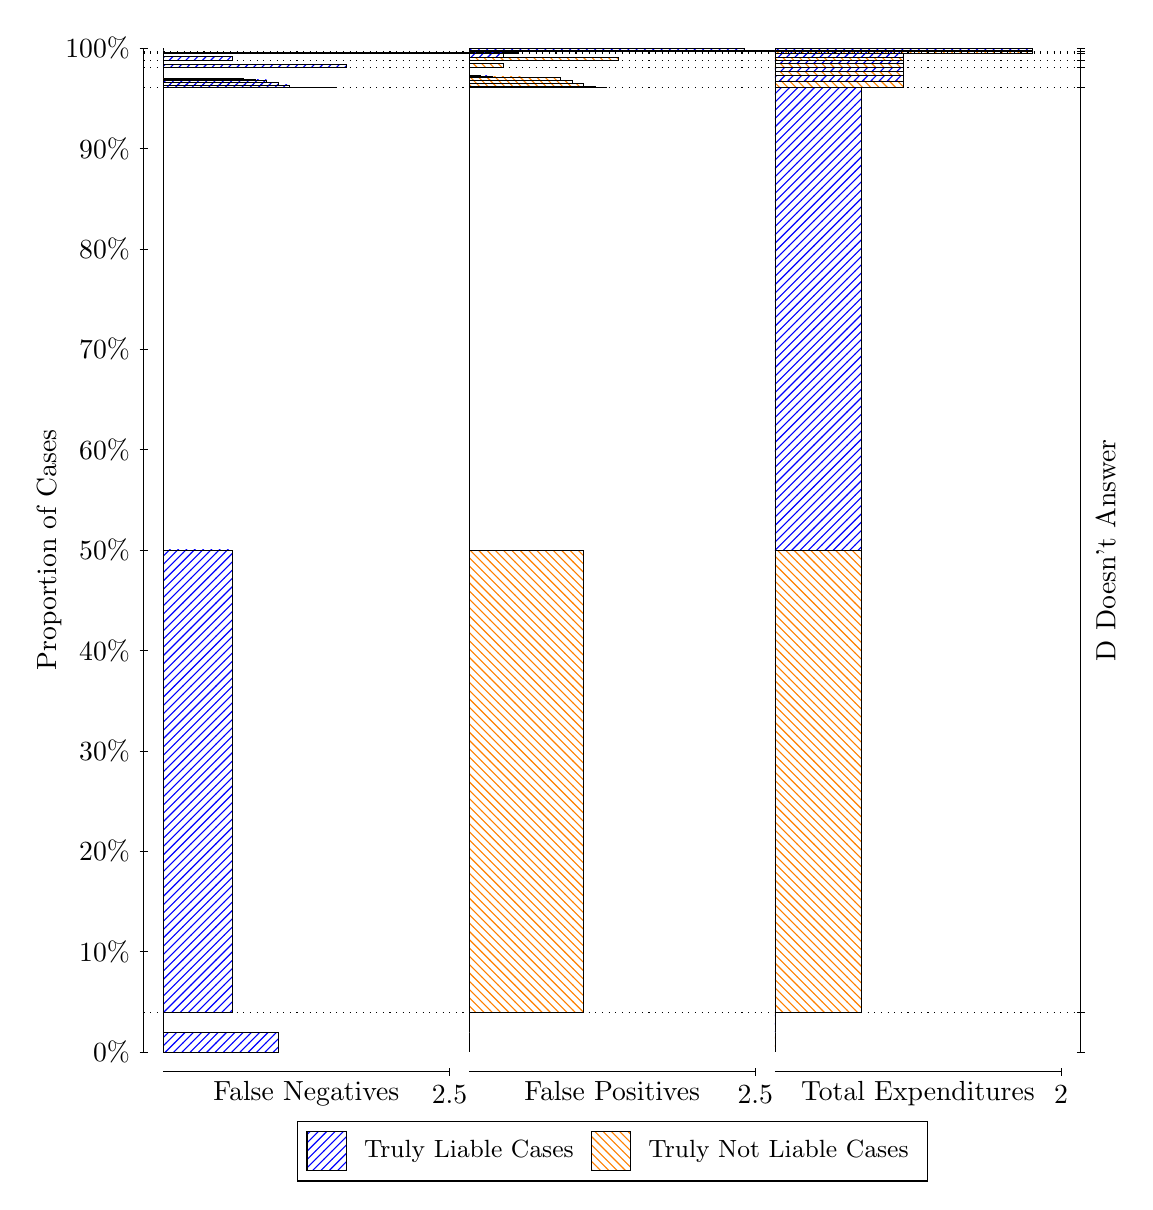
\begin{tikzpicture}
\draw[black, very thin] (1.5,1.75) -- (1.5,14.5);
\node[rotate=90, text=black, anchor=center] at (0.3, 8.125) {Proportion of Cases};
\draw[black, very thin] (1.45,1.75) -- (1.55,1.75);
\node[text=black, anchor=east] at (1.45, 1.75) {0\%};
\draw[black, very thin] (1.45,3.025) -- (1.55,3.025);
\node[text=black, anchor=east] at (1.45, 3.025) {10\%};
\draw[black, very thin] (1.45,4.3) -- (1.55,4.3);
\node[text=black, anchor=east] at (1.45, 4.3) {20\%};
\draw[black, very thin] (1.45,5.575) -- (1.55,5.575);
\node[text=black, anchor=east] at (1.45, 5.575) {30\%};
\draw[black, very thin] (1.45,6.85) -- (1.55,6.85);
\node[text=black, anchor=east] at (1.45, 6.85) {40\%};
\draw[black, very thin] (1.45,8.125) -- (1.55,8.125);
\node[text=black, anchor=east] at (1.45, 8.125) {50\%};
\draw[black, very thin] (1.45,9.4) -- (1.55,9.4);
\node[text=black, anchor=east] at (1.45, 9.4) {60\%};
\draw[black, very thin] (1.45,10.675) -- (1.55,10.675);
\node[text=black, anchor=east] at (1.45, 10.675) {70\%};
\draw[black, very thin] (1.45,11.95) -- (1.55,11.95);
\node[text=black, anchor=east] at (1.45, 11.95) {80\%};
\draw[black, very thin] (1.45,13.225) -- (1.55,13.225);
\node[text=black, anchor=east] at (1.45, 13.225) {90\%};
\draw[black, very thin] (1.45,14.5) -- (1.55,14.5);
\node[text=black, anchor=east] at (1.45, 14.5) {100\%};

\draw[black, very thin] (13.4,1.75) -- (13.4,14.5);
\draw[black, very thin] (13.35,1.75) -- (13.45,1.75);
\node[anchor=west] at (13.35, 1.75) {};
\draw[black, very thin] (13.35,2.2488) -- (13.45,2.2488);
\node[anchor=west] at (13.35, 2.2488) {};
\draw[black, very thin] (13.35,13.998) -- (13.45,13.998);
\node[anchor=west] at (13.35, 13.998) {};
\draw[black, very thin] (13.35,14.252) -- (13.45,14.252);
\node[anchor=west] at (13.35, 14.252) {};
\draw[black, very thin] (13.35,14.34) -- (13.45,14.34);
\node[anchor=west] at (13.35, 14.34) {};
\draw[black, very thin] (13.35,14.437) -- (13.45,14.437);
\node[anchor=west] at (13.35, 14.437) {};
\draw[black, very thin] (13.35,14.461) -- (13.45,14.461);
\node[anchor=west] at (13.35, 14.461) {};
\draw[black, very thin] (13.35,14.5) -- (13.45,14.5);
\node[anchor=west] at (13.35, 14.5) {};

\draw[black, very thin, pattern color=blue, pattern=north east lines] (1.75,1.75) rectangle (3.2033,1.9994);
\draw[black, very thin, pattern color=orange, pattern=north west lines] (1.75,1.9994) rectangle (1.75,2.2488);
\draw[black, very thin, pattern color=blue, pattern=north east lines] (1.75,2.2488) rectangle (2.622,8.126);
\draw[black, very thin, pattern color=orange, pattern=north west lines] (1.75,8.126) rectangle (1.75,13.998);
\draw[black, very thin, pattern color=blue, pattern=north east lines] (1.75,13.998) rectangle (3.93,13.999);
\draw[black, very thin, pattern color=blue, pattern=north east lines] (1.75,13.999) rectangle (3.7847,14);
\draw[black, very thin, pattern color=blue, pattern=north east lines] (1.75,14) rectangle (3.6393,14.002);
\draw[black, very thin, pattern color=blue, pattern=north east lines] (1.75,14.002) rectangle (3.494,14.004);
\draw[black, very thin, pattern color=blue, pattern=north east lines] (1.75,14.004) rectangle (3.3487,14.032);
\draw[black, very thin, pattern color=blue, pattern=north east lines] (1.75,14.032) rectangle (3.2033,14.059);
\draw[black, very thin, pattern color=blue, pattern=north east lines] (1.75,14.059) rectangle (3.058,14.094);
\draw[black, very thin, pattern color=blue, pattern=north east lines] (1.75,14.094) rectangle (2.9127,14.103);
\draw[black, very thin, pattern color=blue, pattern=north east lines] (1.75,14.103) rectangle (2.7673,14.116);
\draw[black, very thin, pattern color=orange, pattern=north west lines] (1.75,14.116) rectangle (1.75,14.252);
\draw[black, very thin, pattern color=blue, pattern=north east lines] (1.75,14.252) rectangle (4.0753,14.289);
\draw[black, very thin, pattern color=orange, pattern=north west lines] (1.75,14.289) rectangle (1.75,14.34);
\draw[black, very thin, pattern color=blue, pattern=north east lines] (1.75,14.34) rectangle (2.622,14.395);
\draw[black, very thin, pattern color=orange, pattern=north west lines] (1.75,14.395) rectangle (1.75,14.437);
\draw[black, very thin, pattern color=blue, pattern=north east lines] (1.75,14.437) rectangle (6.2553,14.443);
\draw[black, very thin, pattern color=orange, pattern=north west lines] (1.75,14.443) rectangle (1.75,14.461);
\draw[black, very thin, pattern color=orange, pattern=north west lines] (1.75,14.461) rectangle (1.75,14.467);
\draw[black, very thin, pattern color=blue, pattern=north east lines] (1.75,14.467) rectangle (1.75,14.5);
\draw[black, very thin, pattern color=orange, pattern=north west lines] (5.6333,1.75) rectangle (5.6333,1.9994);
\draw[black, very thin, pattern color=blue, pattern=north east lines] (5.6333,1.9994) rectangle (5.6333,2.2488);
\draw[black, very thin, pattern color=orange, pattern=north west lines] (5.6333,2.2488) rectangle (7.0867,8.1207);
\draw[black, very thin, pattern color=blue, pattern=north east lines] (5.6333,8.1207) rectangle (5.6333,13.998);
\draw[black, very thin, pattern color=orange, pattern=north west lines] (5.6333,13.998) rectangle (7.3773,14.005);
\draw[black, very thin, pattern color=orange, pattern=north west lines] (5.6333,14.005) rectangle (7.232,14.011);
\draw[black, very thin, pattern color=orange, pattern=north west lines] (5.6333,14.011) rectangle (7.0867,14.052);
\draw[black, very thin, pattern color=orange, pattern=north west lines] (5.6333,14.052) rectangle (6.9413,14.09);
\draw[black, very thin, pattern color=orange, pattern=north west lines] (5.6333,14.09) rectangle (6.796,14.128);
\draw[black, very thin, pattern color=orange, pattern=north west lines] (5.6333,14.128) rectangle (6.6507,14.13);
\draw[black, very thin, pattern color=orange, pattern=north west lines] (5.6333,14.13) rectangle (6.5053,14.132);
\draw[black, very thin, pattern color=orange, pattern=north west lines] (5.6333,14.132) rectangle (6.36,14.133);
\draw[black, very thin, pattern color=orange, pattern=north west lines] (5.6333,14.133) rectangle (6.2147,14.134);
\draw[black, very thin, pattern color=blue, pattern=north east lines] (5.6333,14.134) rectangle (5.924,14.147);
\draw[black, very thin, pattern color=blue, pattern=north east lines] (5.6333,14.147) rectangle (5.7787,14.156);
\draw[black, very thin, pattern color=blue, pattern=north east lines] (5.6333,14.156) rectangle (5.6333,14.252);
\draw[black, very thin, pattern color=orange, pattern=north west lines] (5.6333,14.252) rectangle (6.0693,14.303);
\draw[black, very thin, pattern color=blue, pattern=north east lines] (5.6333,14.303) rectangle (5.6333,14.34);
\draw[black, very thin, pattern color=orange, pattern=north west lines] (5.6333,14.34) rectangle (7.5227,14.383);
\draw[black, very thin, pattern color=blue, pattern=north east lines] (5.6333,14.383) rectangle (6.0693,14.437);
\draw[black, very thin, pattern color=orange, pattern=north west lines] (5.6333,14.437) rectangle (5.6333,14.455);
\draw[black, very thin, pattern color=blue, pattern=north east lines] (5.6333,14.455) rectangle (5.6333,14.461);
\draw[black, very thin, pattern color=orange, pattern=north west lines] (5.6333,14.461) rectangle (10.575,14.467);
\draw[black, very thin, pattern color=blue, pattern=north east lines] (5.6333,14.467) rectangle (9.1213,14.5);
\draw[black, very thin, pattern color=orange, pattern=north west lines] (9.5167,1.75) rectangle (9.5167,1.9994);
\draw[black, very thin, pattern color=blue, pattern=north east lines] (9.5167,1.9994) rectangle (9.5167,2.2488);
\draw[black, very thin, pattern color=orange, pattern=north west lines] (9.5167,2.2488) rectangle (10.607,8.1207);
\draw[black, very thin, pattern color=blue, pattern=north east lines] (9.5167,8.1207) rectangle (10.607,13.998);
\draw[black, very thin, pattern color=orange, pattern=north west lines] (9.5167,13.998) rectangle (11.152,14.084);
\draw[black, very thin, pattern color=blue, pattern=north east lines] (9.5167,14.084) rectangle (11.152,14.157);
\draw[black, very thin, pattern color=orange, pattern=north west lines] (9.5167,14.157) rectangle (11.152,14.207);
\draw[black, very thin, pattern color=blue, pattern=north east lines] (9.5167,14.207) rectangle (11.152,14.252);
\draw[black, very thin, pattern color=orange, pattern=north west lines] (9.5167,14.252) rectangle (11.152,14.303);
\draw[black, very thin, pattern color=blue, pattern=north east lines] (9.5167,14.303) rectangle (11.152,14.34);
\draw[black, very thin, pattern color=orange, pattern=north west lines] (9.5167,14.34) rectangle (11.152,14.383);
\draw[black, very thin, pattern color=blue, pattern=north east lines] (9.5167,14.383) rectangle (11.152,14.437);
\draw[black, very thin, pattern color=orange, pattern=north west lines] (9.5167,14.437) rectangle (12.787,14.455);
\draw[black, very thin, pattern color=blue, pattern=north east lines] (9.5167,14.455) rectangle (12.787,14.461);
\draw[black, very thin, pattern color=orange, pattern=north west lines] (9.5167,14.461) rectangle (12.787,14.467);
\draw[black, very thin, pattern color=blue, pattern=north east lines] (9.5167,14.467) rectangle (12.787,14.5);
\draw[black, dotted] (1.5,2.2488) -- (13.4,2.2488);
\draw[black, dotted] (1.5,13.998) -- (13.4,13.998);
\draw[black, dotted] (1.5,14.252) -- (13.4,14.252);
\draw[black, dotted] (1.5,14.34) -- (13.4,14.34);
\draw[black, dotted] (1.5,14.437) -- (13.4,14.437);
\draw[black, dotted] (1.5,14.461) -- (13.4,14.461);
\draw[black, very thin] (1.75,1.5) -- (5.3833,1.5);
\node[text=black, anchor=north] at (3.5667, 1.5) {False Negatives};
\draw[black, very thin] (5.3833,1.45) -- (5.3833,1.55);
\node[text=black, anchor=north] at (5.3833, 1.45) {2.5};

\draw[black, very thin] (5.6333,1.5) -- (9.2667,1.5);
\node[text=black, anchor=north] at (7.45, 1.5) {False Positives};
\draw[black, very thin] (9.2667,1.45) -- (9.2667,1.55);
\node[text=black, anchor=north] at (9.2667, 1.45) {2.5};

\draw[black, very thin] (9.5167,1.5) -- (13.15,1.5);
\node[text=black, anchor=north] at (11.333, 1.5) {Total Expenditures};
\draw[black, very thin] (13.15,1.45) -- (13.15,1.55);
\node[text=black, anchor=north] at (13.15, 1.45) {2};


\node[text=black, centered, rotate=90] at (13.72, 8.1233) {D Doesn't Answer};






\draw (7.449999999999999,1.5) node[draw=none] (baseCoordinate) {};
\begin{scope}[align=center]
        \matrix[scale=0.5, draw=black, below=0.5cm of baseCoordinate, nodes={draw}, column sep=0.1cm]{
            \node[rectangle, draw, minimum width=0.5cm, minimum height=0.5cm, pattern color=blue, pattern=north east lines] {}; &
            \node[draw=none, font=\small, text=black] (B) {Truly Liable Cases}; &
            \node[rectangle, draw, minimum width=0.5cm, minimum height=0.5cm, pattern color=orange, pattern=north west lines] {}; &
            \node[draw=none, font=\small, text=black] (B) {Truly Not Liable Cases}; \\
            };
\end{scope}

\end{tikzpicture}
\end{document}